\documentclass[12pt,a4paper]{article}
\usepackage[utf8]{inputenc}
\usepackage{amsmath}
\usepackage{amsfonts}
\usepackage{amssymb}

\usepackage{placeins}
\usepackage{cmap} % для кодировки шрифтов в pdf
\usepackage[T1]{fontenc}
\usepackage{hhline}
\usepackage[unicode]{hyperref}
\usepackage{multirow}
\usepackage{array}
\usepackage{amsmath}
\usepackage{bm}
\usepackage{textcomp}
\usepackage[russian]{babel}
\usepackage{graphicx} % для вставки картинок
\usepackage{amssymb,amsfonts,amsmath,amsthm} % математические дополнения от АМС
\usepackage{indentfirst} % отделять первую строку раздела абзацным отступом тоже
% Поля
\usepackage{geometry}
\geometry{left=2cm}
\geometry{right=1.5cm}
\geometry{top=2.4cm}
\geometry{bottom=2.cm}

%%%%%%%%%%%%%%%%%%%%%%%%%%%%%%%     

\linespread{1.5} % полуторный интервал
\frenchspacing




\begin{document}
	
	\begin{titlepage}
		
		\begin{center}
			\begin{large}
				Санкт-Петербургский Политехнический университет\\ Петра Великого\\
				Физико-механический институт\\
			\end{large}
			\vspace{0.2cm}
			Высшая школа прикладной математики и вычислительной физики\\
			
		\end{center}
		
		\vspace{3cm}
		\begin{center}
			\textbf{Отчёт\\ по лабораторной работе №3\\ по дисциплине\\ "Анализ данных с интервальной \\неопределенностью"}
		\end{center}
		
		\vspace{3cm}
		
		\vbox{%
			\hfill%
			\vbox{%
				\hbox{Выполнил студент:}%
				\hbox{\break}
				\hbox{Иванов Андрей Игоревич,}%
				\hbox{группа 5040102$\backslash$20201}%
				\hbox{\break}
				\hbox{\break}
				\hbox{Проверил:}
				\hbox{\break}
				\hbox{к.ф.-м.н., доцент}
				\hbox{Баженов Александр Николаевич}
			}%
		} 
		\vfill
		
		\begin{center}
			Санкт-Петербург, 2023
		\end{center}
	
	\end{titlepage}
	\tableofcontents
	\newpage
	
	\listoffigures
	\newpage
	
	\section{Постановка задачи}
            Дано множество вещественных выборок, соответствующих показаниям -0.45, -0.35, -0.25, -0.15, 0.05, 0.05, 0.15, 0.25, 0.35, 0.45. Необходимо:
            \begin{itemize}
                \item Сформировать интервальную выборку по имеющимся данным и выборку остатков по полученной интервальной;
                \item Найти точечную линейную регрессию для обеих выборок;
                \item Построить информационное множество коэффициентов регрессии (решить задачу восстановления зависимости) для обеих выборок
                \item Построить коридор совместных зависимостей задачи восстановления для обеих выборок
                \item Построить диаграмму статусов для выборки остатков
            \end{itemize}
	\newpage
	
	\section{Теория}
            \subsection{Формирование интервальной выборки}
                Дано множество из N выборок вещественных чисел $\mathbf{\{X_i\}}_{i=1}^N$. По этому множеству формируется интервальная выборка по следующему принципу:
                \begin{equation}
                    X = \{(min(\mathbf{X_i}), max(\mathbf{X_i}))\ | \mathbf{X_i} \in \mathbf{\{X_i\}}_{i=1}^N \}\}
                \end{equation}

            \subsection{Формирование выборки остатков}
                Дана интервальная выборка Y и ее регрессионная модель. Выборка остатков формируется следующим образом:
                \begin{equation}
                    X_{res} = \{y_i - (\beta_0 + \beta_1 \cdot x_i) | y_i \in Y, x_i \in \{values\}\}
                \end{equation}
                
            \subsection{Точечная линейная регрессия}
                Рассматривается задача восстановления зависимости для выборки
                $ (X, \textbf(Y))$, $ X = \{x_i\}_{i=1}^{n}, \textbf{Y} = \{\textbf{y}_i\}_{i=1}^{n} $,
                $ x_i $ - точеный, $ \textbf{y}_i $ - интервальный.
                Пусть искомая модель задана в классе линейных функций:
            
                \begin{equation}
                    y = \beta_0 + \beta_1 x
                \end{equation}
            
                Поставим задачу оптимизацию для нахождения точечных оценок
                параметров $ \beta_0, \beta_1 $.
            
                \begin{equation}
                    \begin{gathered}
                        \sum_{i = 1}^{m}w_{i} \to \min \\
                        \text{mid}\textbf{y}_{i} - w_{i} \cdot \text{rad}\textbf{y}_{i} \leq \beta_0 + \beta_1 x \leq \text{mid}\textbf{y}_{i} + w_{i} \cdot \text{rad}\textbf{y}_{i} \\
                        w_{i} \geq 0, i = 1, ..., m \\
                        {w_i}, \beta_0, \beta_1 - ?
                    \end{gathered}
                    \label{e:task}
                \end{equation}
                
                Задачу можно решить методами линейного программирования.
            
                \subsection{Информационное множество}
                \textbf{Информационным множеством} задачи восстановления зависимости
                будем называть множество значений всех параметров зависимости,
                совместных с данными в каком-то смысле. 
            
                \textbf{Коридором совместных зависимостей} задачи восстановления зависимости
                называется многозначное множество отображений $ \Upsilon $, сопоставляющее
                каждому значению аргумента $ x $ множество
                
                \begin{equation}
                    \Upsilon(x) = \bigcup_{\beta \in \Omega} f(x, \beta)
                \end{equation}
                , где $ \Omega $ - информационное множество, $ x $ - вектор переменных, $ \beta $ - вектор оцениваемых параметров. 

            \subsection{Классификация измерений}
                Измерения можно классифицировать следующим образом.
                Измерения, добавление которых к выборке не приводит к модификации модели, называются \textsl{внутренними}.
                Те, которые изменяют модель, называются \textsl{внешними}.
                Измерения, которые определяют какую-либо границу информационного множества, называются \textsl{граничными}.
                \textsl{Выбросами} называются те измерения, которые делают информационное множество пустым.
                Граничные измерения - подмножество внутренних, выбросы - внешних.
            
                Для удобства анализа взаимоотношения информационных множеств работу с ними заменяют
                на анализ взаимоотношения интересующего интервального измерения и интервального прогнозируемого
                значения модели (коридора совместных значений).
            
                \subsection{Взаимные отношения интервалов наблюдения и прогнозного интервала модели}
                \quad Существует несколько характеристик, определяющих это взаимоотношение.
            
                \textsl{Размахом (плечом)} называется следующее отношение:
                \begin{equation}
                    l(x, \textbf{y}) = \frac{\Upsilon(x)}{rad(\textbf{y})}
                \end{equation}
            
                \textsl{Относительным остатком} называется отношение:
                \begin{equation}
                    r(x, \textbf{y}) = \frac{mid(\textbf{y}) - mid(\Upsilon(x))}{rad(\textbf{y})}
                \end{equation}
                здесь $ x $ - точечное значение, $ \textbf{y} $ - интервальное значение интересующей величины (отклик $ x $),
                $ \Upsilon(x) $ - интервальная оценка интересующей величины (значение коридора совместных значений).
            
                Для внутренних наблюдений выполняется неравенство:
                \begin{equation}
                    |r(x, \textbf{y})| \leq 1 - l(x, \textbf(y))
                \end{equation}
                
                В случае равенства 
                \begin{equation}
                    |r(x, \textbf{y})| = 1 - l(x, \textbf(y))
                \end{equation}
                измерение будет граничным.
            
                Выбросы определяются неравенством
                \begin{equation}
                    |r(x, \textbf{y})| > 1 + l(x, \textbf{y})
                \end{equation}
                
	\newpage
	
	\section{Реализация}
		Лабораторная работа выполнена на языке Python 3.10 с помощью загружаемых пакетов NumPy, MatPlotLib, SciPy. Исходный код лабораторной работы находится на \href{https://github.com/Drusiand/SPbSTU_Interval_Analysis.git}{GitHub репозитории}.
	\newpage
	
	\section{Результаты}  
            \subsection{Интервальная выборка}
                \begin{figure}[h!]
                    \centering
                    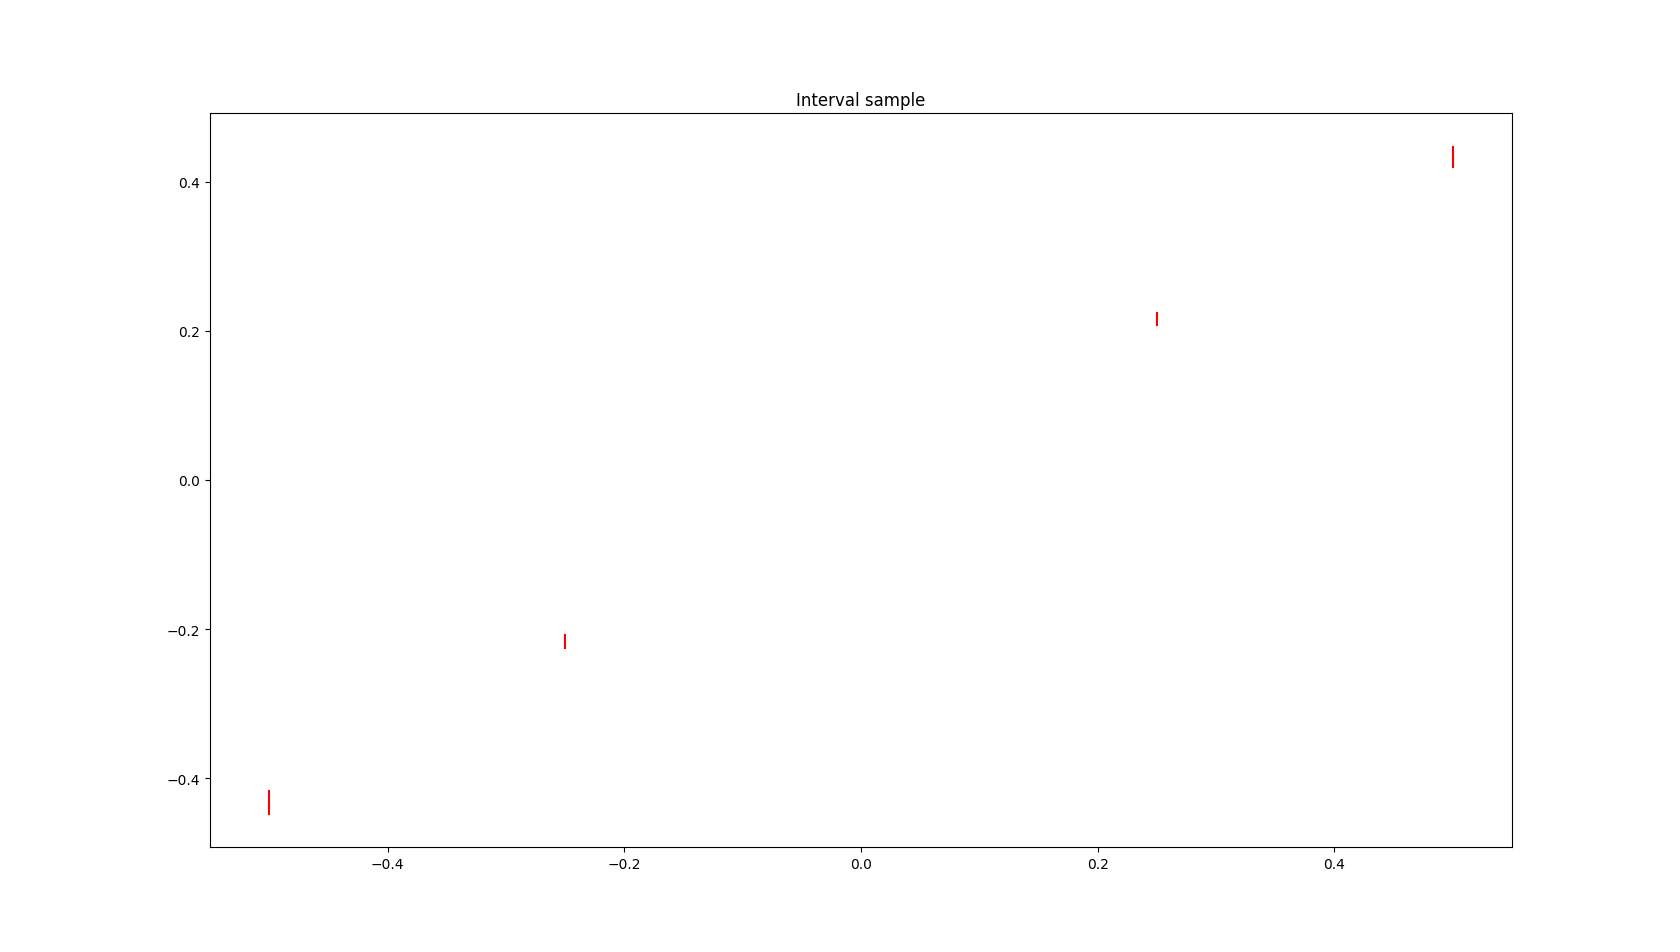
\includegraphics[width=0.95\linewidth]{sample_plot.png}
                    \caption{График интервальной выборки}
                \end{figure}
                \FloatBarrier
                
                \begin{figure}[h!]
                    \centering
                    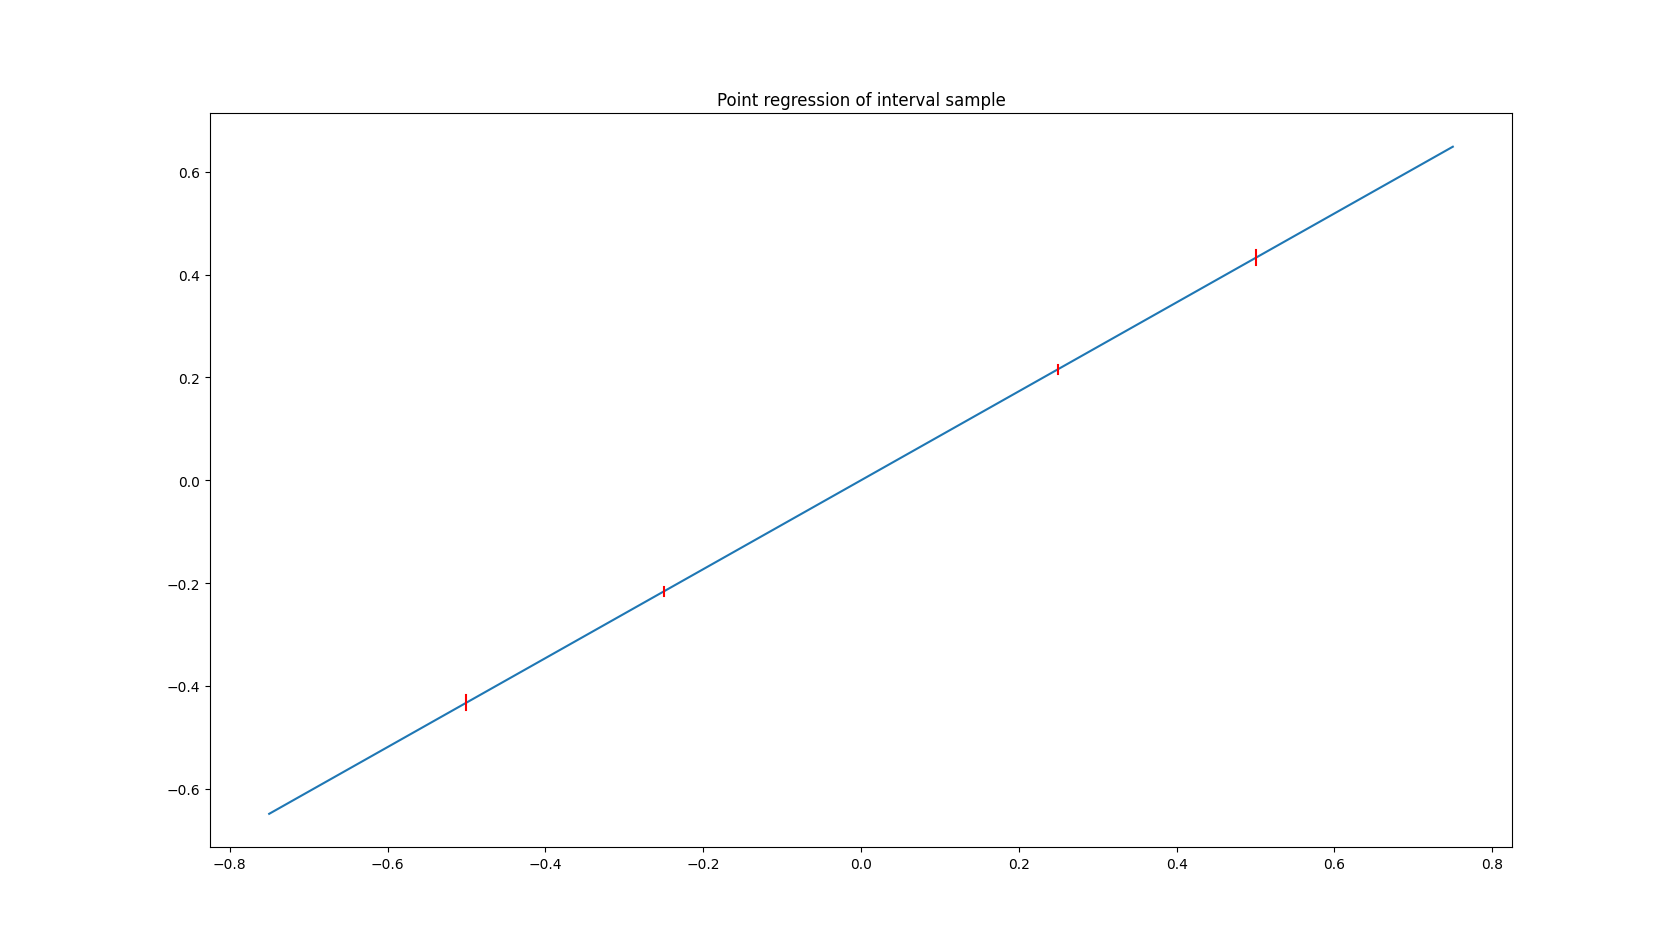
\includegraphics[width=0.95\linewidth]{sample_regr.png}
                    \caption{Точечная регрессия интервальной выборки}
                \end{figure}
                \FloatBarrier
                
                \begin{figure}[h!]
                    \centering
                    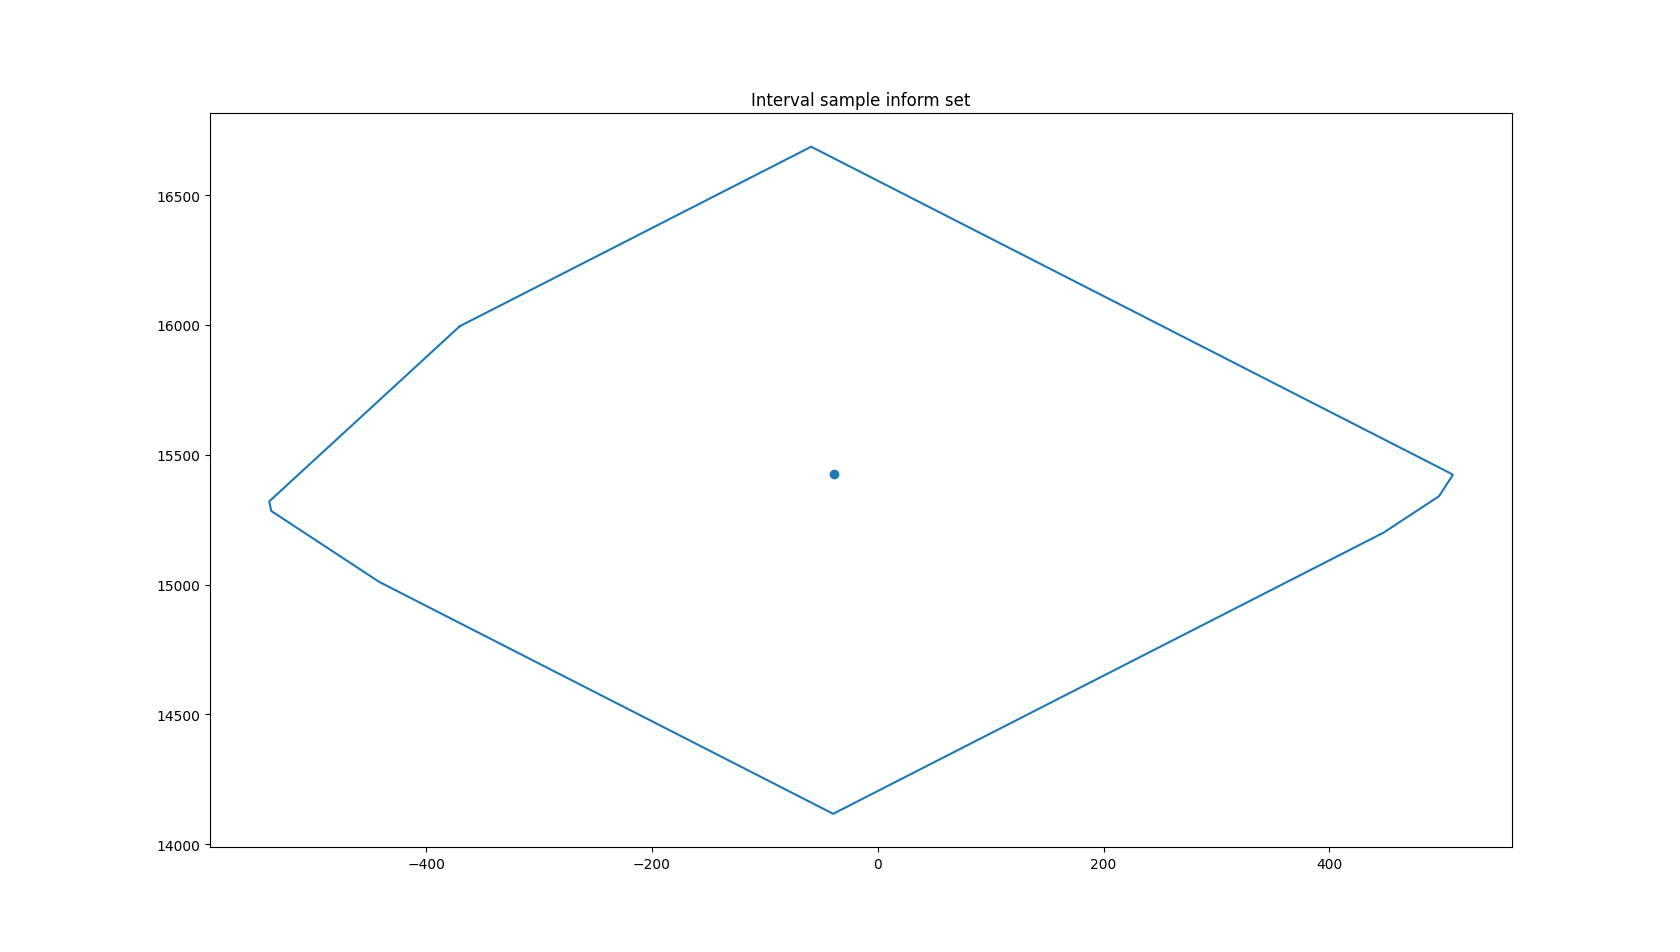
\includegraphics[width=0.95\linewidth]{sample_inf_set.png}
                    \caption{Информационное множество для интервальной выборки}
                \end{figure}
                \FloatBarrier
    
                \begin{figure}[h!]
                    \centering
                    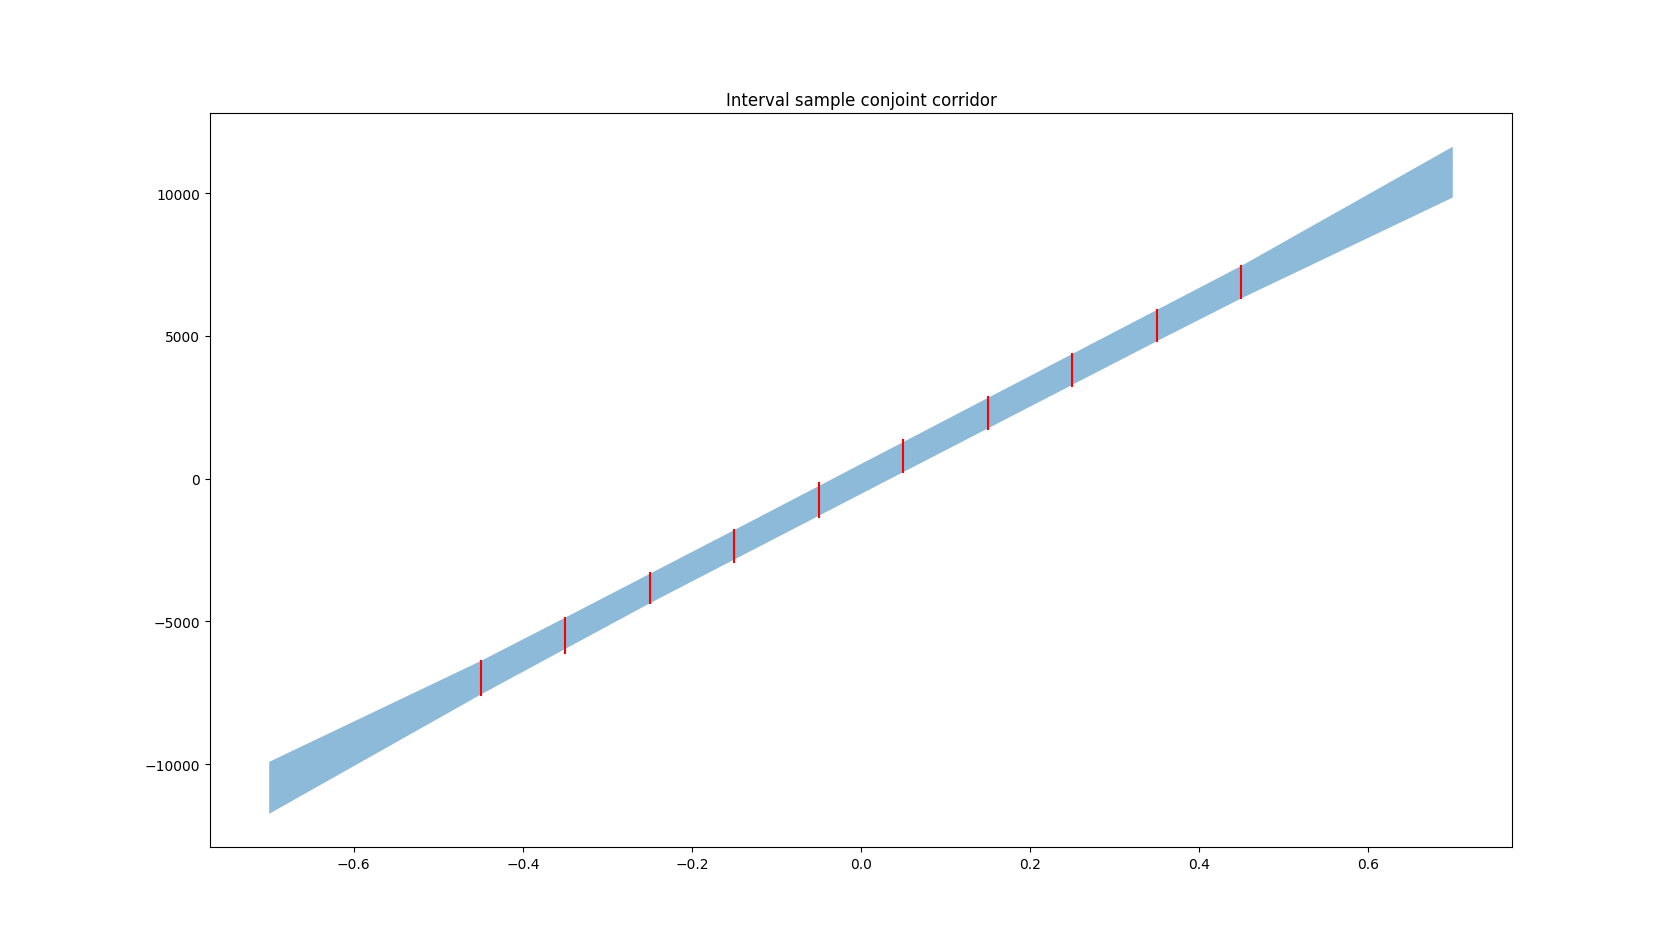
\includegraphics[width=0.95\linewidth]{sample_cor.png}
                    \caption{Коридор совместных значений для интервальной выборки}
                \end{figure}
                \FloatBarrier

                Ниже приведена таблица, описывающая итоговую интервальную выборку
                \begin{center}
                    \begin{tabular}{|c|c|c|}
                    \hline
                        \textbf{Набор данных} & $\mathbf{\underline{x_i}}$ & $\mathbf{\overline{x_i}}$\\
                        \hline
                        -0.45V\_sp115.dat&-7568&-6392\\
                        \hline
                        -0.35V\_sp196.dat&-6117&-4872\\
                        \hline
                        -0.25V\_sp403.dat&-4369&-3307\\
                        \hline
                        -0.15V\_sp155.dat&-2906&-1804\\
                        \hline
                        -0.05V\_sp465.dat&-1338&-155\\
                        \hline
                        0.05V\_sp321.dat&227&1335\\
                        \hline
                        0.15V\_sp135.dat&1721&2843\\
                        \hline
                        0.25V\_sp135.dat&3235&4368\\
                        \hline
                        0.35V\_sp300.dat&4812&5907\\
                        \hline
                        0.45V\_sp1014.dat&6313&7450\\
                        \hline
                    \end{tabular}
                \end{center}
                Искомая модель принимает вид:
                \begin{equation}
                    y = -39.03125 + 15424.374999 \cdot x
                \end{equation}
            
            \subsection{Выборка остатков}
                \begin{figure}[h!]
                    \centering
                    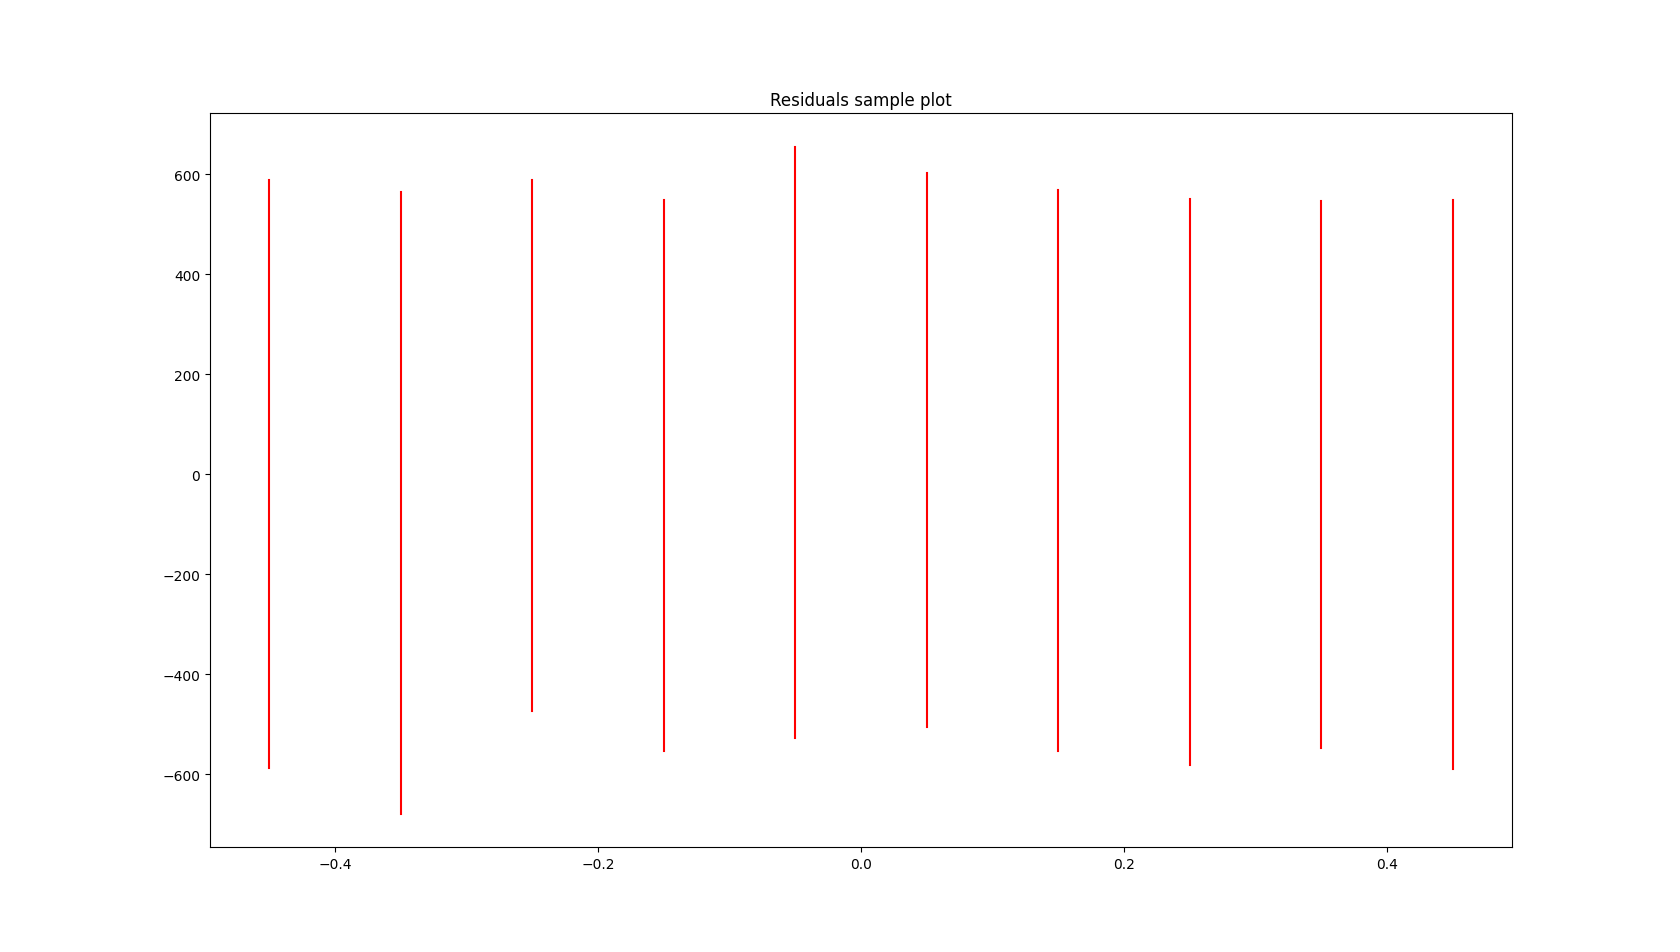
\includegraphics[width=0.95\linewidth]{res_plot.png}
                    \caption{График выборки остатков}
                \end{figure}
                \FloatBarrier
                
                \begin{figure}[h!]
                    \centering
                    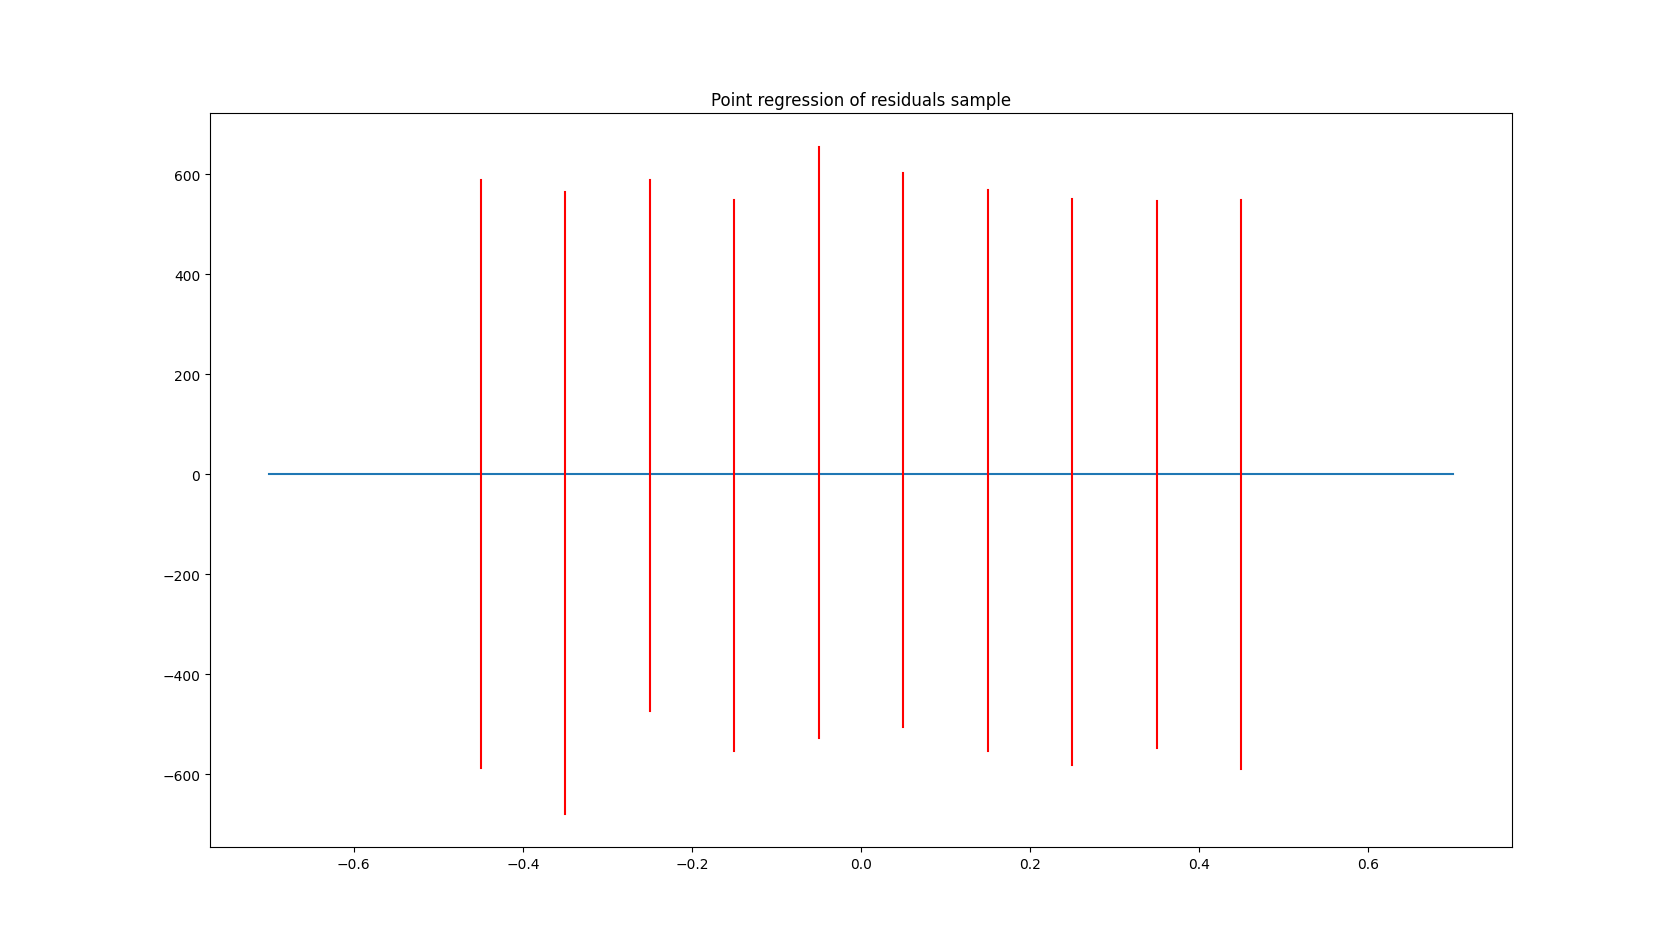
\includegraphics[width=0.95\linewidth]{res_regr.png}
                    \caption{Точечная регрессия выборки остатков}
                \end{figure}
                \FloatBarrier
                
                \begin{figure}[h!]
                    \centering
                    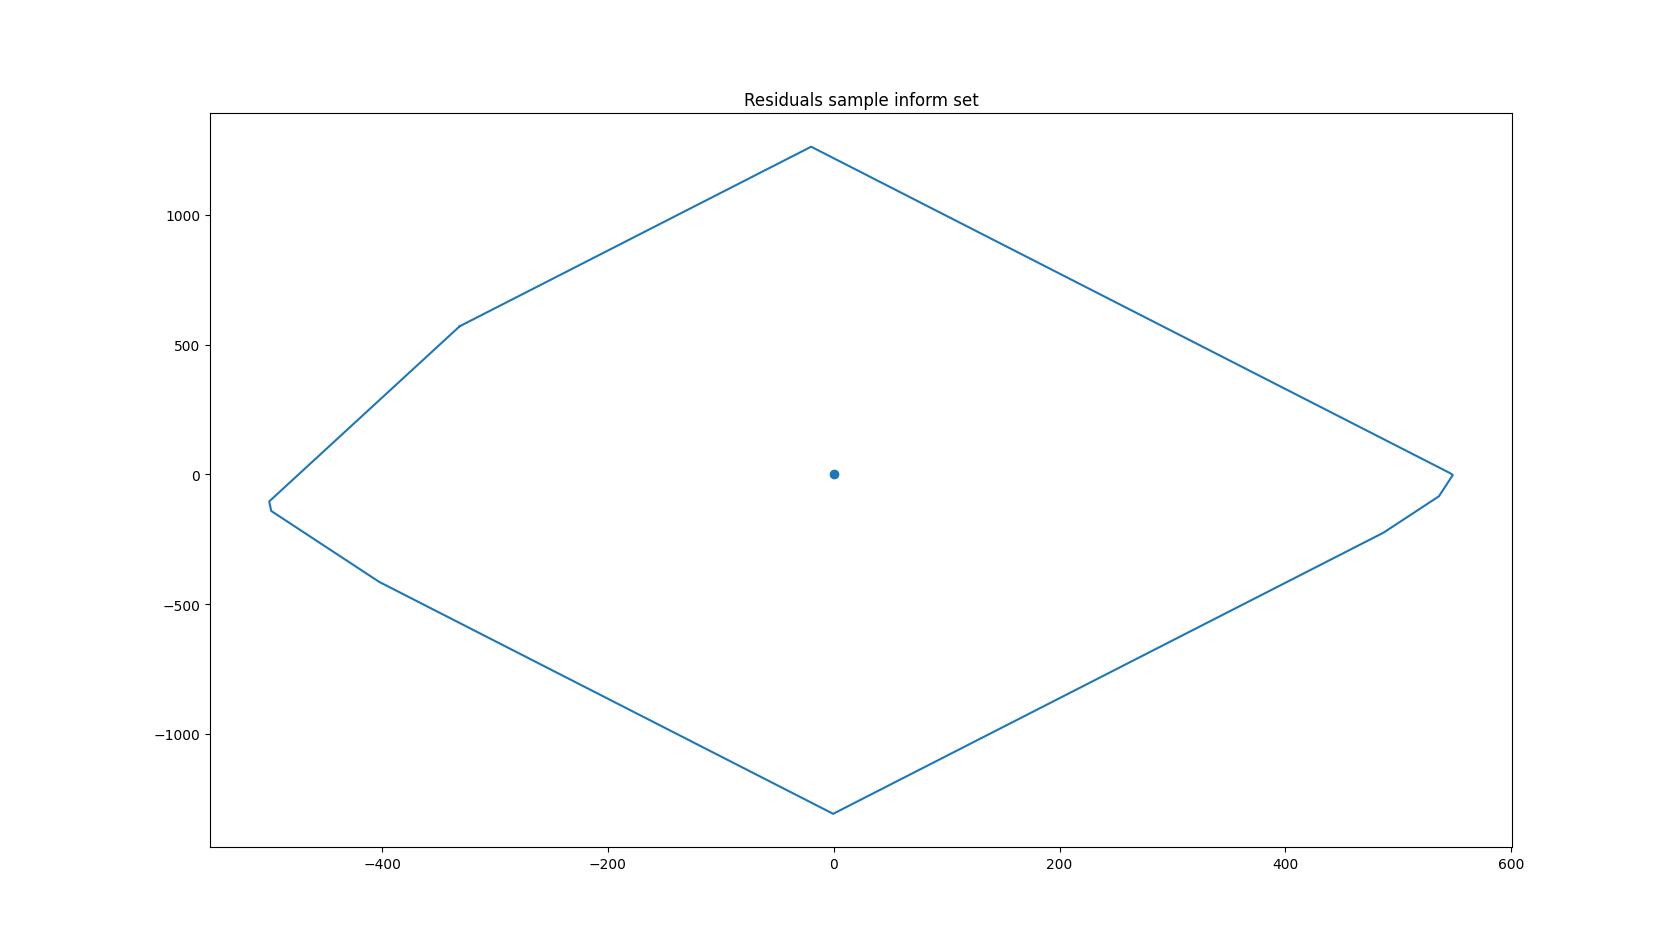
\includegraphics[width=0.95\linewidth]{res_inf_set.png}
                    \caption{Информационное множество для выборки остатков}
                \end{figure}
                \FloatBarrier
                
                \begin{figure}[h!]
                    \centering
                    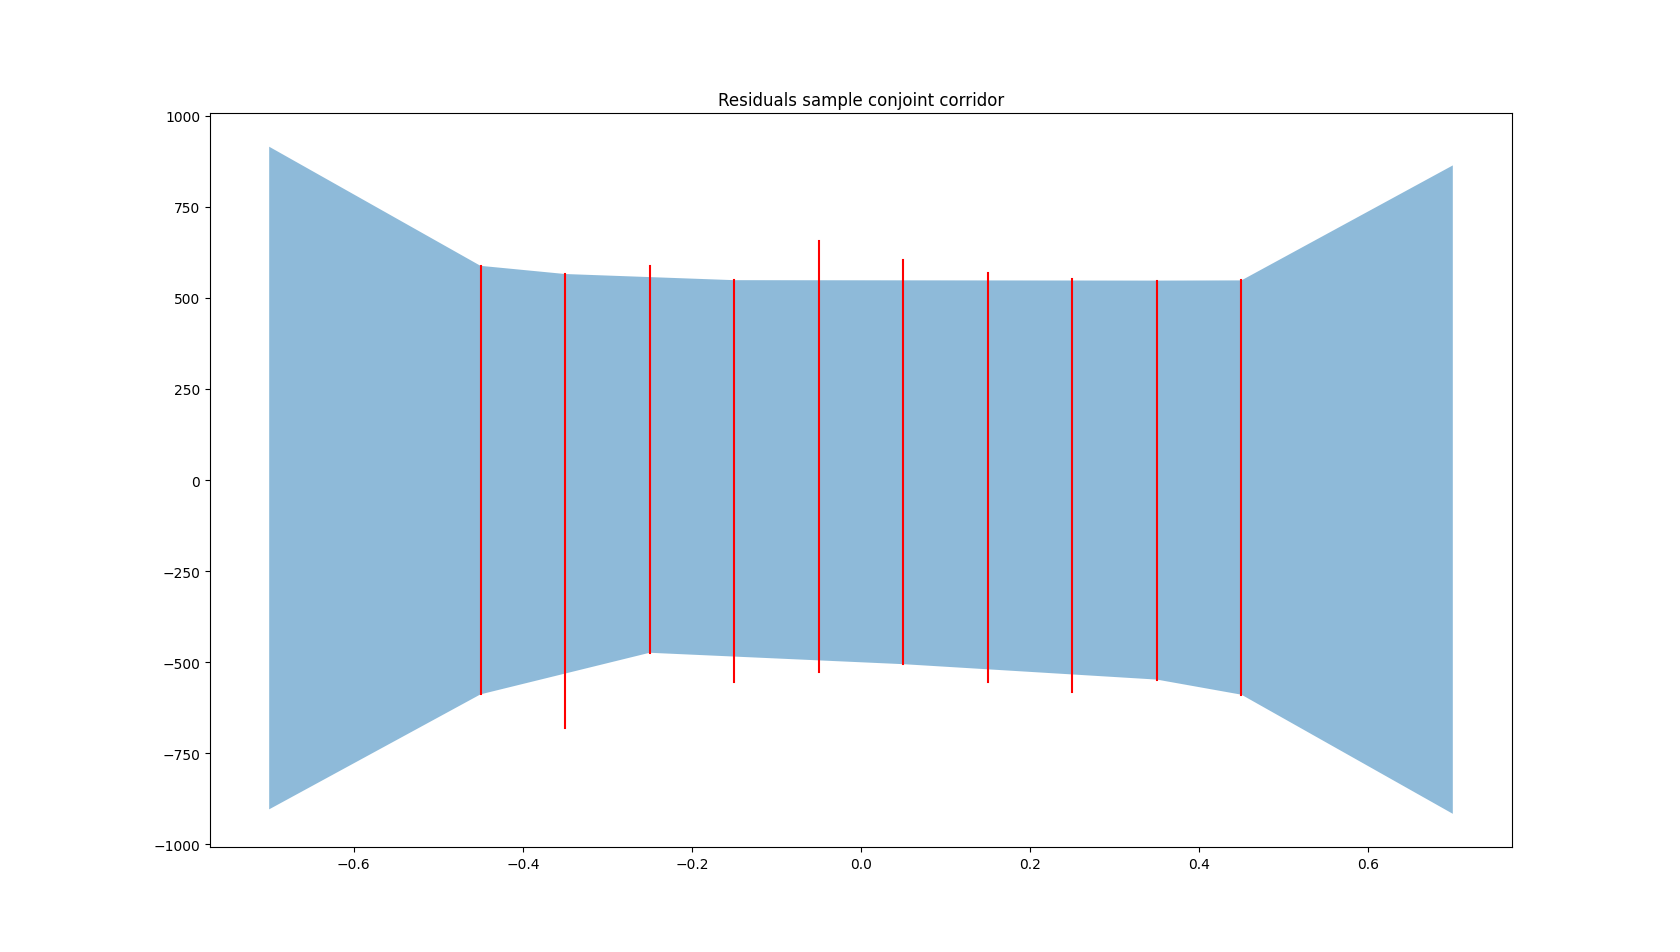
\includegraphics[width=0.95\linewidth]{res_cor.png}
                    \caption{Коридор совместных значений для выборки остатков}
                \end{figure}
                \FloatBarrier

                \begin{figure}[h!]
                    \centering
                    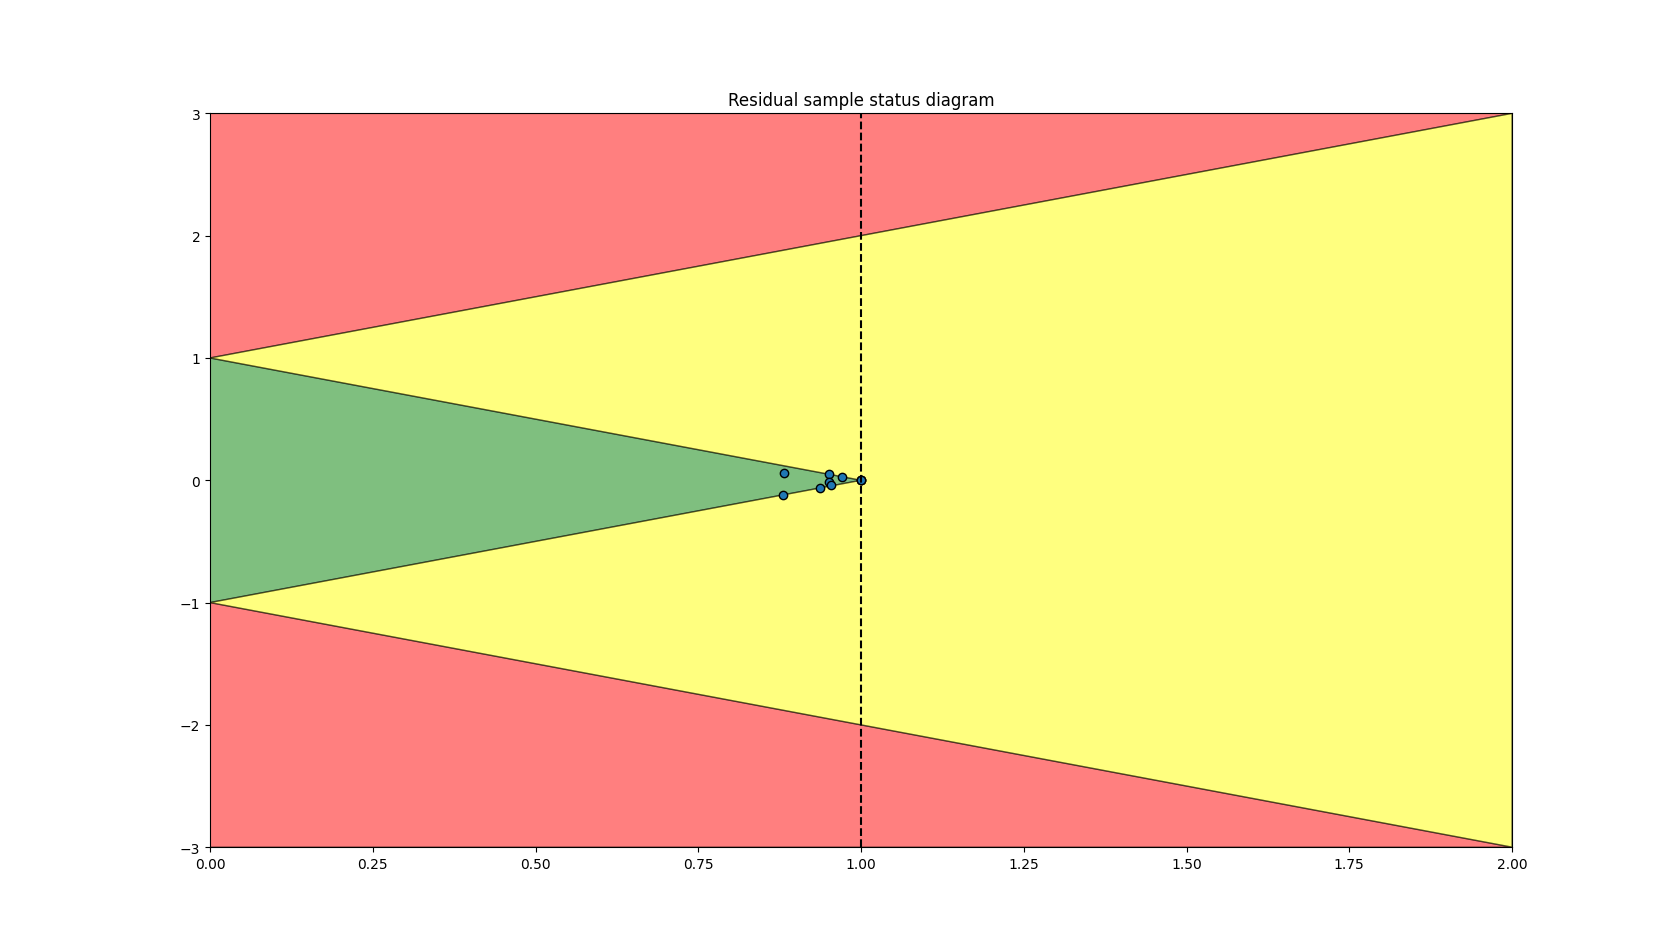
\includegraphics[width=0.95\linewidth]{res_status.png}
                    \caption{Диаграмма статусов для выборки остатков}
                \end{figure}
                \FloatBarrier

                Ниже приведена таблица, описывающая выборку остатков:
                \begin{center}
                    \begin{tabular}{|c|c|c|}
                    \hline
                        \textbf{Набор данных} & $\mathbf{\underline{x_i}}$ & $\mathbf{\overline{x_i}}$\\
                        \hline
                        -0.45V\_sp115.dat&-588.000000538862&587.999999461138]\\
                        \hline
                        -0.35V\_sp196.dat&-679.4375004133717&565.5624995866283\\
                        \hline
                        -0.25V\_sp403.dat&-473.8750002878801&588.1249997121199\\
                        \hline
                        -0.15V\_sp155.dat&-553.3125001623894&548.6874998376106\\
                        \hline
                        -0.05V\_sp465.dat&-527.7500000368989&655.2499999631011\\
                        \hline
                        0.05V\_sp321.dat &-505.1874999114084&602.8125000885916\\
                        \hline
                        0.15V\_sp135.dat &-553.6249997859177&568.3750002140823\\
                        \hline
                        0.25V\_sp135.dat &-582.062499660427&550.937500339573\\
                        \hline
                        0.35V\_sp300.dat &-547.4999995349363&547.5000004650637\\
                        \hline
                        0.45V\_sp1014.dat&-588.937499409446&548.062500590554\\
                        \hline
                        \hline
                    \end{tabular}
                \end{center}
                Искомая модель принимает вид:
                \begin{equation}
                    y = 0.000001\cdot x
                \end{equation}
               
        \clearpage
	\newpage

\end{document}